 	\subsection{Classement des cas d'utilisation} 
 	{\renewcommand{\arraystretch}{1.5} % distance entre les lignes
 	{\setlength{\tabcolsep}{1cm} % distance entre les colonnes
	\begin{tabular}{|l|c|r|}
		\hline
		\textbf{Cas d'utilisation} & \textbf{Priorité} & \textbf{Risque} \\
		\hline
		Création et Gestion de compte & Haute & Moyen \\
		\hline
		Types de connexion & Haute & Moyen \\
		\hline
		Gestion du panier & Haute & Haut \\
		\hline
		Consultation et Mise en vente d'objets & Haute & Haut \\
		\hline
		Messagerie & Basse & Bas \\
		\hline
		Paiement & Basse & Moyen \\
		\hline
		Recherche d'objets & Haute & Haut \\
		\hline
		Valorisation des comptes & Moyenne & Bas \\
		\hline
	\end{tabular} \\
	\subsection{Modèle du Domaine}
	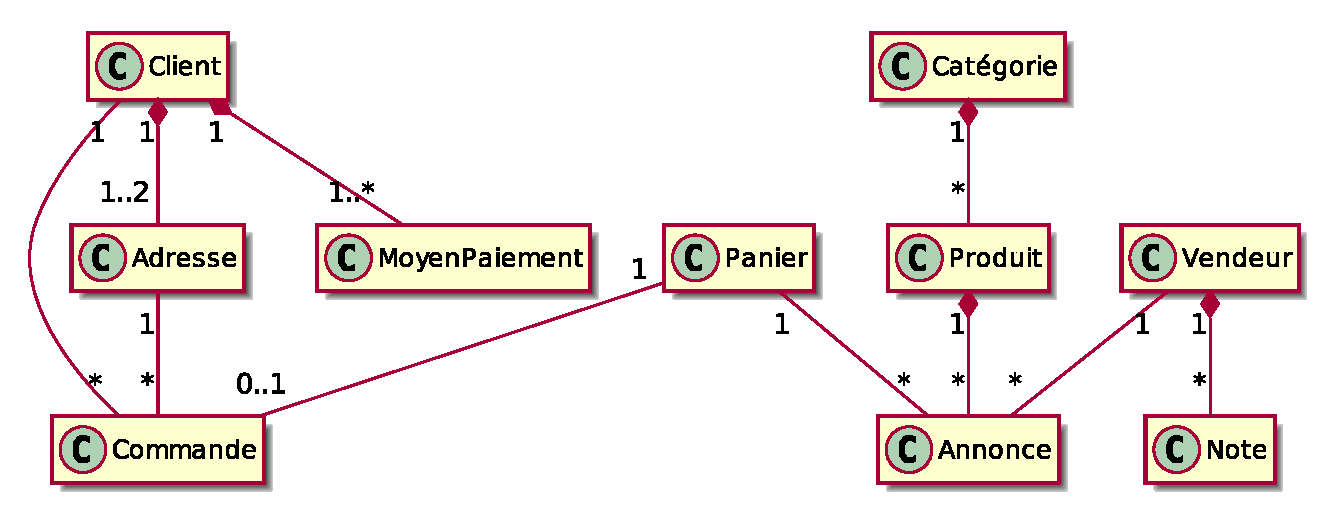
\includegraphics[width=15cm]{Images/MD} 

	\subsection{Diagramme de navigation}
	
	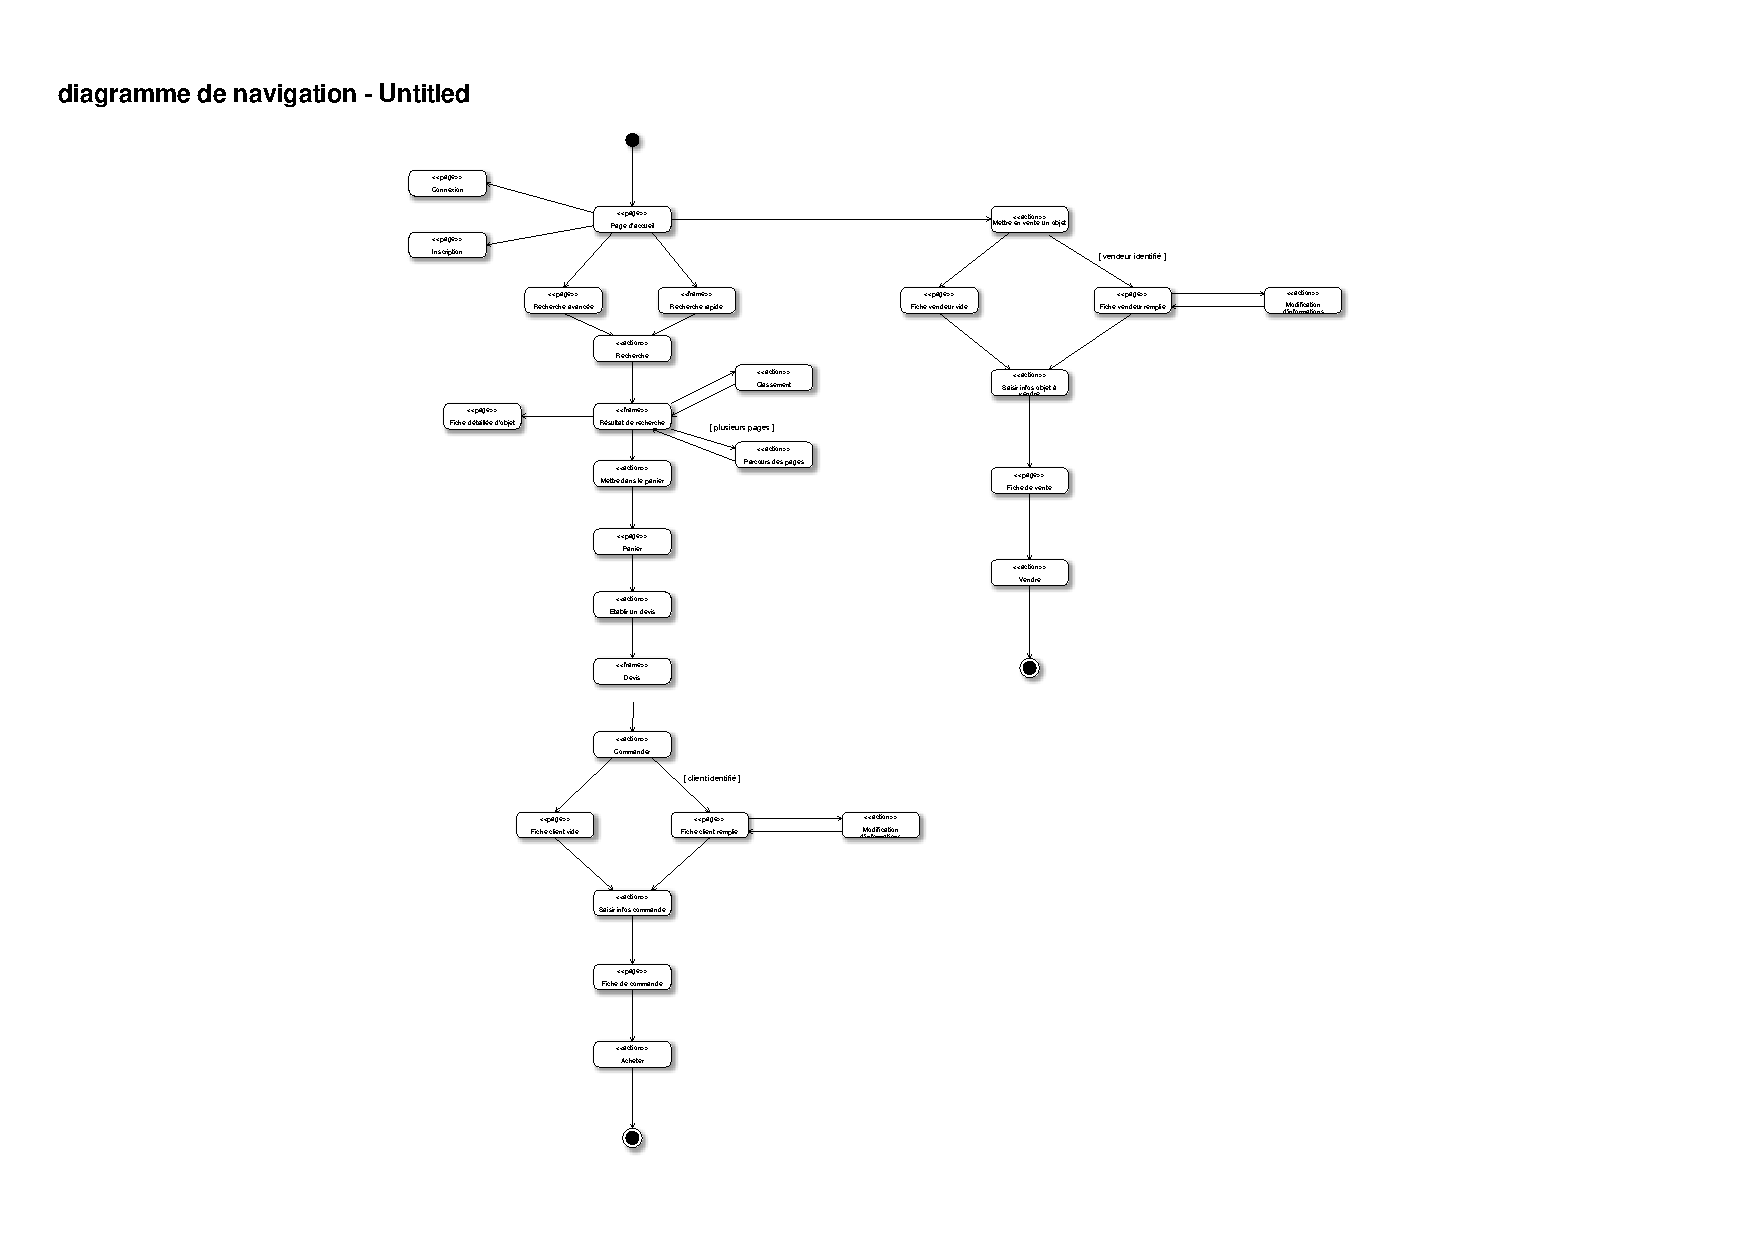
\includegraphics[trim = 6cm 1.5cm 5cm 2.2cm, clip]{Images/DN}
	
	\subsection{Identification des acteurs}
	
	Les acteurs humains pour le site Web sont :
	\begin{itemize}
		\item l'administrateur : en charge du bon fonctionnement (validation des annonces et des messages échangés) et de la maintenance du site   
		\item l'utilisateur non connecté : visiteur du site, n'a pas de compte 
		\item l'utilisateur connecté : possède un compte, peut acheter et vendre des objets
	\end{itemize}
	
	\subsection{Diagrammes de Cas d'Utilisation}
	\begin{itemize}
		\item DCU de l'Administrateur \\ 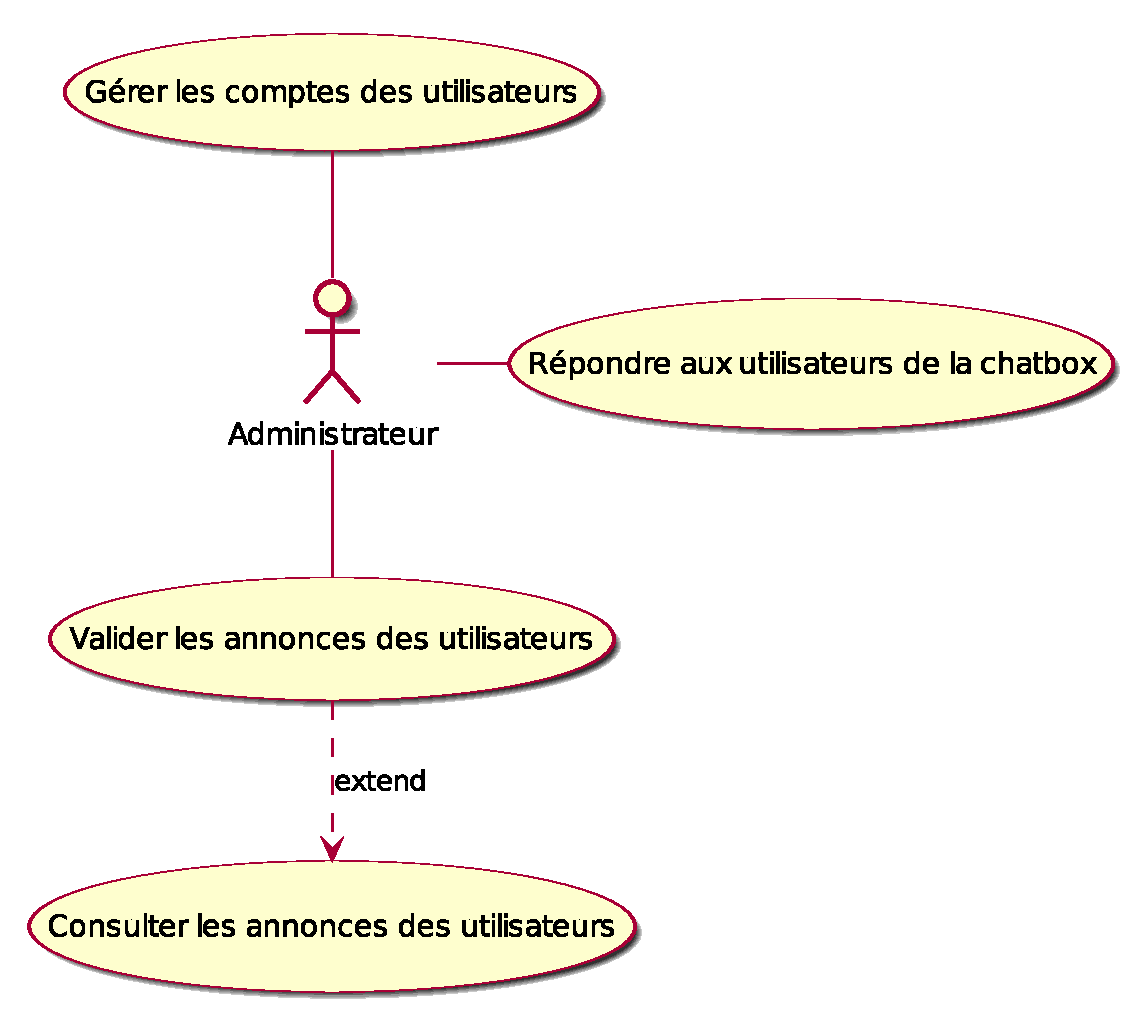
\includegraphics[height=10cm,width=15cm]{Images/DCU_Administrateur}
		\newpage
		\item DCU de l'Utilisateur Non Connecté \\
		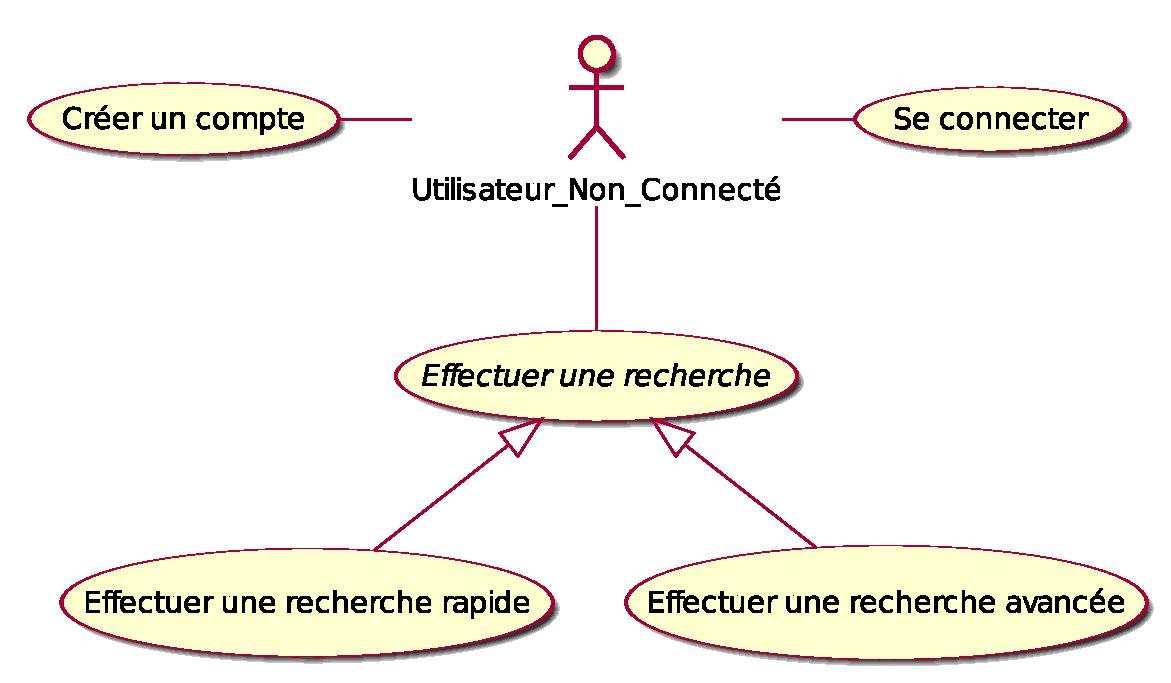
\includegraphics[height=7cm,width=15cm]{Images/DCU_UtilisateurNonConnecte} 
		\item DCU de l'Utilisateur Connecté \\
		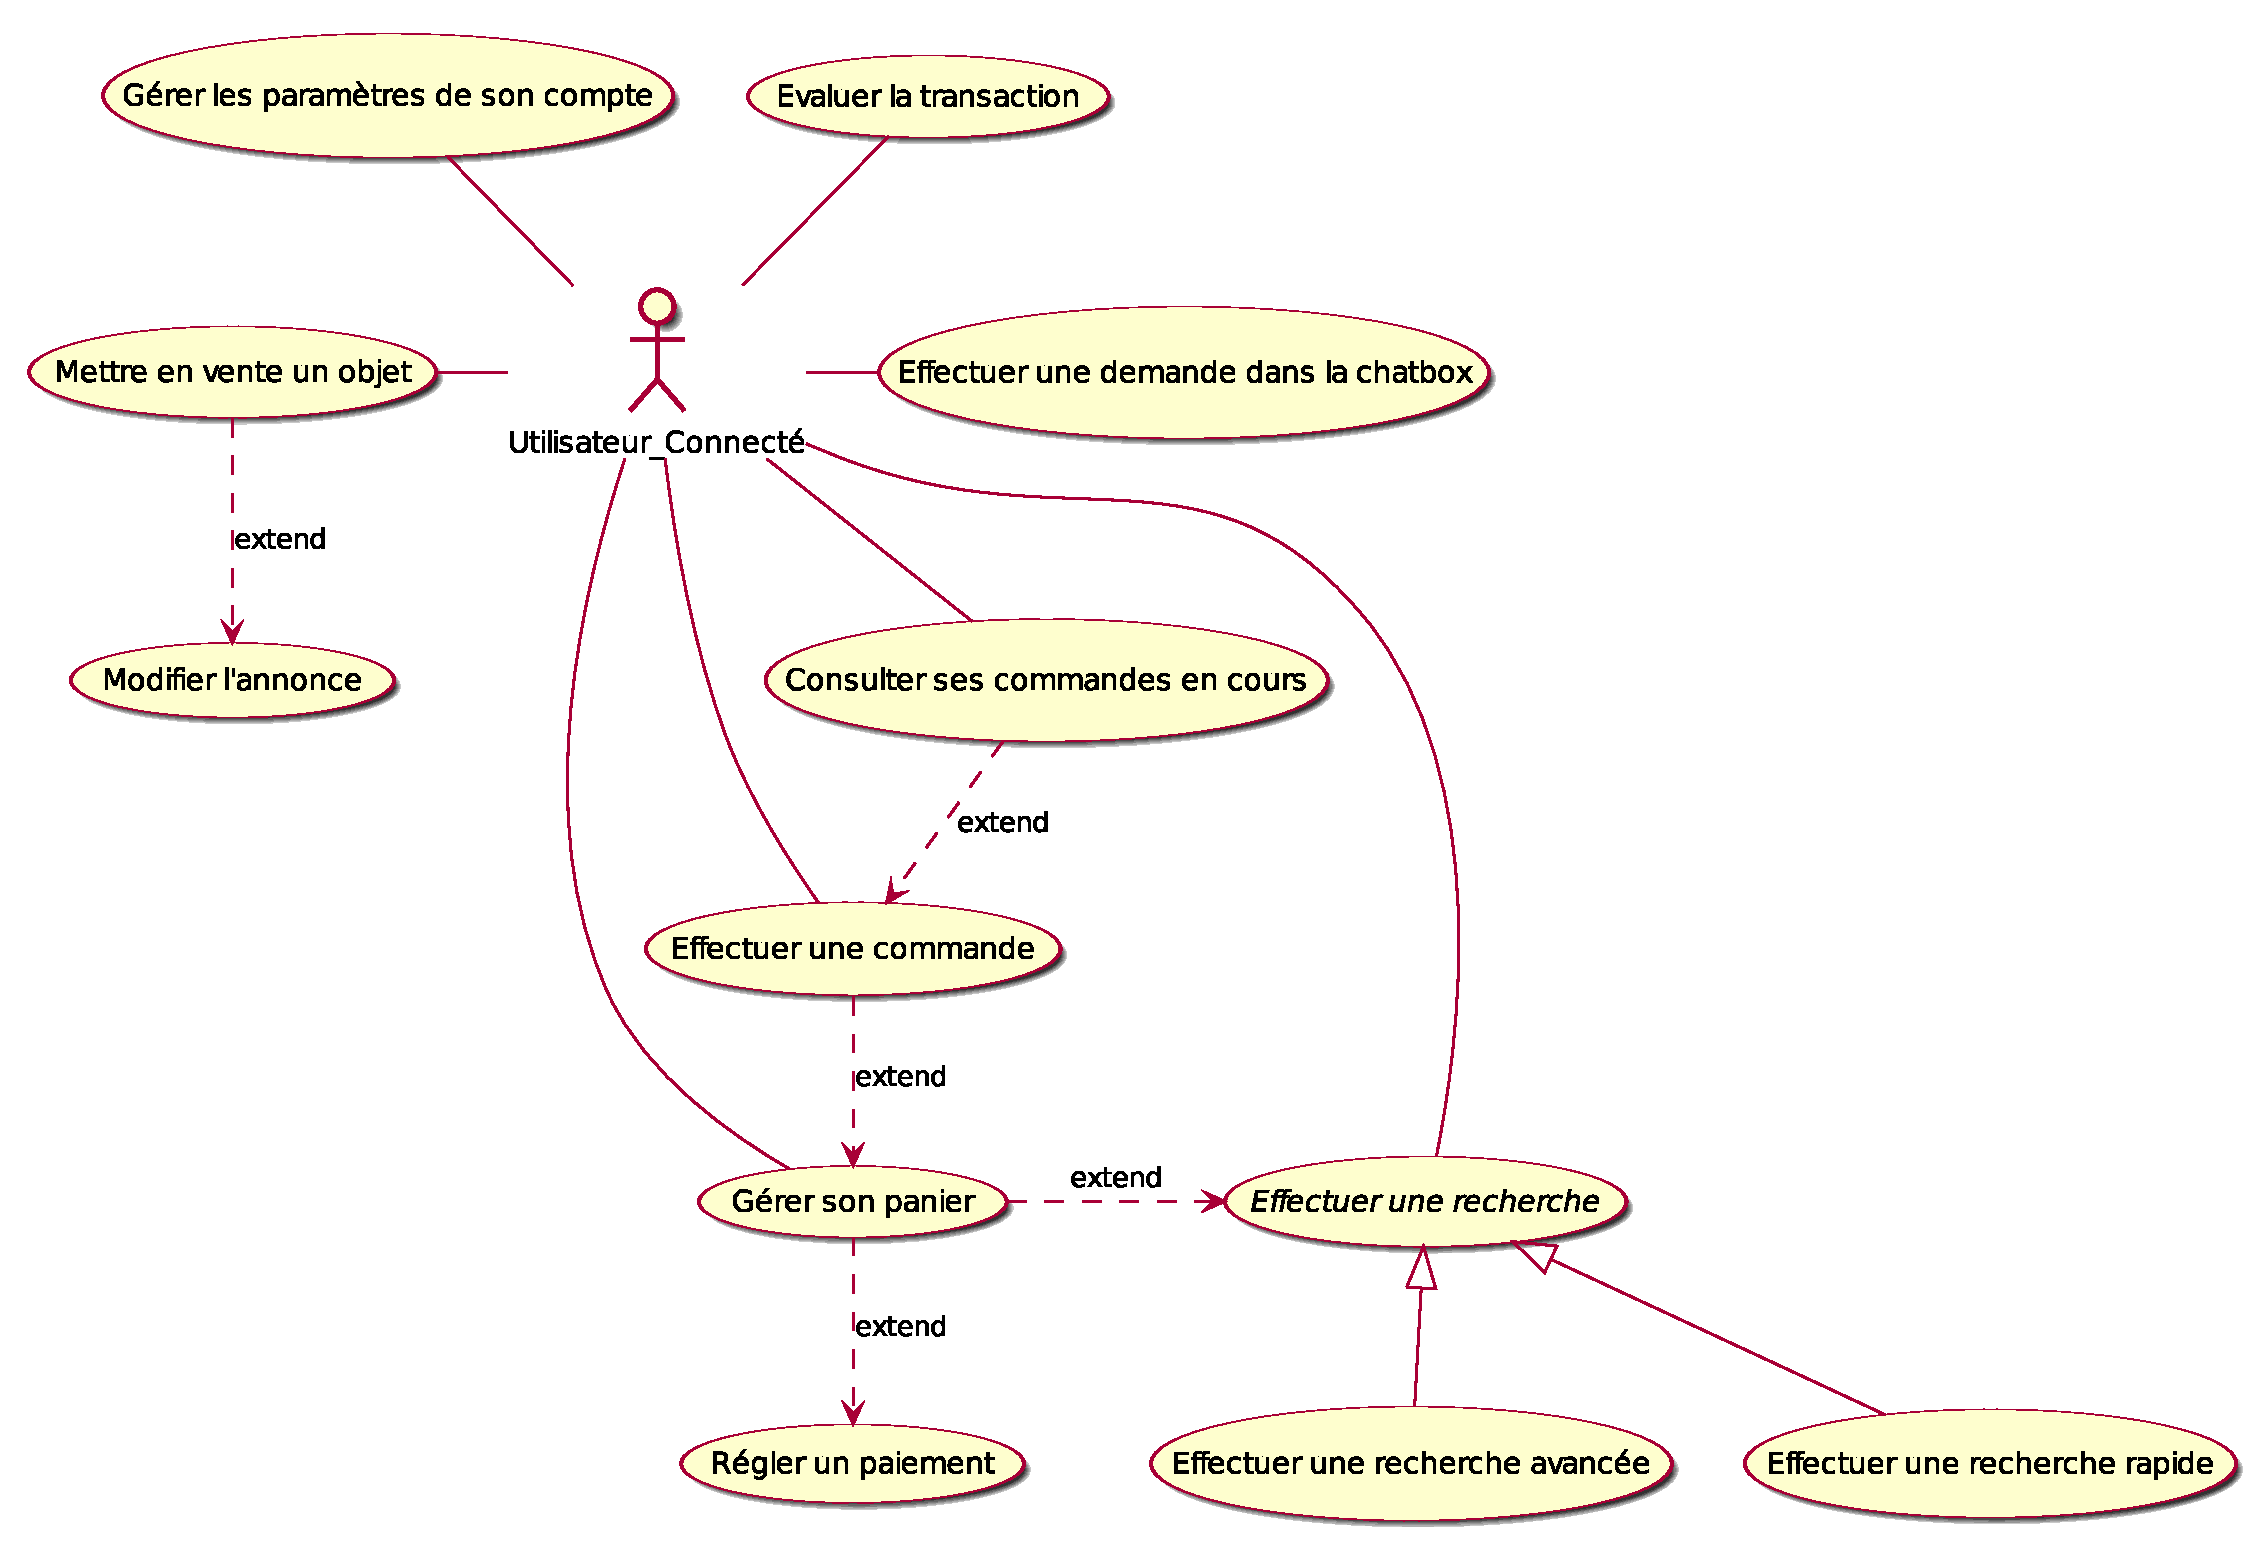
\includegraphics[width=17cm]{Images/DCU_UtilisateurConnecte} 
	\end{itemize}